\begin{figure}
	\centering
	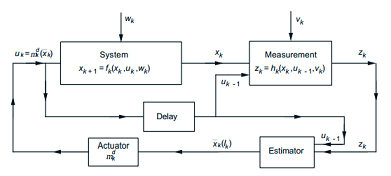
\includegraphics[scale=0.7]{CEC}
\end{figure}



Como podemos ver en este reporte hizo una revisión técnica de los modelos de regresión basados en procesos gaussianos, revisando desde los aspectos más básicos hasta otros bastante complejos. Sin embargo hay muchos otros temas relacionados que pueden ser interesantes, entre ellas las diferentes aplicaciones a problemas reales de modelación y como técnicas de resolución de problemas de diferente naturaleza. Una de las principales aplicaciones de los procesos gaussianos es utilizarlos para estimar las funciones de un modelo de espacio de estado \cite{2}\cite{3}\cite{4}\cite{5} o de un modelo dinámico \cite{58}. Otras aplicaciones incluyen modelar ecuaciones diferenciales \cite{35}, problemas de control óptimo \cite{34}, o incluso como modelos de volatilidad \cite{63}, con ruidos heterocedásticos \cite{59}\cite{61}, ruido en la entrada \cite{57}, como un proceso de cópulas \cite{62} o de volatilidad multidimensional \cite{64}. Otra importante aplicación es la de optimización Bayesiana \cite{67}\cite{68}, donde se basa en modelar la función a optimizar como un proceso gaussiano, de forma que todos los cálculos para escoger el próximo punto a evaluar se realizan utilizando el proceso gaussiano, que se actualiza una vez que se evalúa la función verdadera. Esto permite reducir considerablemente la cantidad de veces que se evalúa la función objetivo, que en muchos casos es muy costosa computacionalmente, tal como es el caso de la función de verosimilitud. Incluso este enfoque nos permite realizar optimización sin utilizar derivadas, reduciendo aún más la complejidad computacional.

Como pudimos ver en todo el reporte, la alta complejidad computaciones que tiene el entrenamiento de los procesos gaussianos obliga a buscar aproximaciones eficientes con el fin de poder aplicarlos a problemas de alta dimensionalidad. Además del enfoque de los modelos \emph{sparse} que fue estudiado en el capítulo 4, también es posible atacar directamente la inversión de la matriz de covarianza de forma eficiente. En \cite{18} se estudia el caso común en donde la función de kernel produce matrices de covarianza que pueden factorizarse de forma jerárquica en productos de matrices de bajo rango, llegando a reducir la complejidad computacion, bajo los supuestos adecuados, de $O\left( n^{3}\right) $ a $O\left( n\log ^{2}n\right) $. Por otro lado, en \cite{19} se propone un método iterativo que estima directamente la matriz de precisión, pero sin invertir directamente la matriz de covarianza. El método se aprovecha del hecho que los procesos gaussianos no puede representar las independencia condicionales entre variables, por lo que dado un grafo no dirigido que codifica las independencias condicionales entre las variables, el método es capaz de calcular la matriz de precisión en un tiempo $O\left( nc^{3}\right) $, donde $c$ es el tama\~{n}o del mayor clique del \emph{junction tree} asociado al grafo.

Otra área muy interesante es dise\~{n}ar modelos más expresivos que los procesos gaussianos por si sólos. En el capítulo 6 vimos diferentes modelos jerárquicos que incluyen procesos gaussianos dentro de sus elementos, pero existen otras formas de construir procesos con propiedades interesantes, tales como el producto de procesos gaussianos \cite{60} que produce procesos no estacionarios, o construir un proceso de Poisson cuyas intensidades se modelan con un proceso gaussiano \cite{65}.Otras propuestas incluyen utilizar otras leyes finito dimensionales, construyendo así procesos de \emph{Wishart }generalizados \cite{56}, el cual se puede comparar como un modelo \emph{GARCH} pero bayesiano y no paramétrico. En \cite{66} los autores proponen un modelo a partir de la distribución \emph{Student-t}, construyendo así un proceso
aleatorio en donde un proceso gaussiano se puede ver como un caso particular. Todos estos modelos y otra generalizaciones buscan crear modelos más flexibles, pero el costo que se debe asumir es un aumento en la complejidad computacional, llegando a expresiones donde en muchos casos no tienen solución analítica, por lo que las técnicas variacionales son altamente utilizadas para proponer reglas de inferencia y
entrenamiento de los modelos. Para la incorporación de otras funciones de probabilidades es interesante revisar los métodos de \emph{kernels} \emph{embedding}\cite{8}\cite{9}\cite{10}\cite{11}, en donde es posible estimar distribuciones generales de forma no paramétrica, ya que la familia de distribuciones se mapea a un espacio \emph{RKHS}, en donde las reglas de marginalización y condicionamiento de distribuciones se expresan de forma explícita.

Espero que este reporte sirva como guía introductoria a los procesos gaussianos y que pueda ser utilizado como texto en algún curso avanzado. Mi intención es seguir trabajando en este reporte, de forma que en un tiempo más tenga la calidad suficiente para publicarlo como un libro, agregando algunos métodos y modelos desarrollados por mi y mis colaboradores. Quiero agradecer a Felipe Tobar, por todo el tiempo y la dedicación que ha invertido en mi, ya que gracias a él conocí los procesos gaussianos, lo que me llevó a cambiar mi linea de investigación del doctorado a este tema que me cautivó.


\section{Modelos Bayesianos Jerárquicos}

Ahora estamos en condiciones de definir la clase de modelos conocidos como \emph{Bayesian Networks}, para luego enfocarnos en su extensión \emph{Dynamic Bayesian Networks}, la cual nos permite modelar series de tiempo. Todas las definiciones, propiedades y algoritmos a continuación son
tomadas principalmente de los textos \cite{DBN-StateOfArt}, \cite
{DBN-LearningDBN} y \cite{DBN-Murphy}.

\subsection{Redes Bayesianas}

Una red bayesiana (\emph{Bayesian Network}) es un tipo de modelo gráfico dirigido, en donde los nodos se interpretan como las variables de los modelos, y los arcos se interpretan como dependencias directas entre las variables. El grafo inducido es un \emph{DAG} (\emph{Directed Acyclic Graph}), ya que las dependencias no pueden formar ciclos, y en algunos casos más simples es un árbol (\emph{tree}) o poliárbol (\emph{polytree}). La idea general de las redes bayesianas es codificar eficientemente la función de probabilidad conjunta, evitando suposiciones de independencia erróneas, utilizando suposiciones de independencia condicional. Veamos a
continuación la definición formal.

\begin{figure}
	\centering
	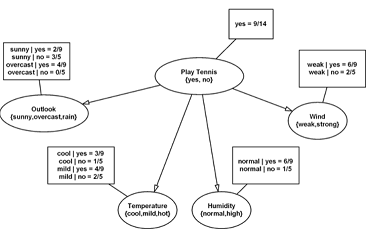
\includegraphics[scale=0.7]{bayesian-network}
\end{figure}

\begin{definition}
Sea $\mathcal{X}$ un conjunto de variables aleatorias, y sea $\mathcal{V\subset X\times X}$ un conjunto de arcos tales que la estructura inducida $G=(\mathcal{X},\mathcal{V})$ sea un grafo dirigido acíclico. Para cada $X\in \mathcal{X}$ denotamos al conjunto de padres de $X$ como $\Pi \lbrack X]=\{Y\in\mathcal{X}\ |\ (Y,X)\in \mathcal{V}\},$ y denotemos $\mathbb{P}_{\Pi }(X)=$ $\mathbb{P}(X\ |\ \Pi \lbrack X])$ a su función de  probabilidad condicional. Sea $\Theta=\{\mathbb{P}_{\Pi }(X)|\ X\in \mathcal{X}\}$, entonces se dice que el par $B=(G,\Theta )$ es una red Bayesiana.
\end{definition}

La eficiencia de codificación de las redes bayesianas se logra gracias a la propiedad de independencia condicional de los nodos dado sus padres, ya que con sólo calcular y almacenar sus funciones de probabilidades condicionales, podemos calcular fácilmente la función de probabilidad conjunta. La siguiente proposición nos muestra la forma de esta relación.

\begin{proposition}
Dada $B=(G,\Theta)$ una red bayesiana, con $\mathcal{X}=\{X_{1},...,X_{N}\}$, entonces la función de probabilidad conjunta cumple que\ $\mathbb{P}(X_{1},...,X_{N})=\prod\limits_{i=1}^{N}\mathbb{P}_{\Pi }(X_{i}).$
\end{proposition}

Una vez teniendo a nuestra disposición la función de probabilidad conjunta, somos capaces de \emph{preguntar} y \emph{agregar} información a medida que sea necesario. Por ejemplo, si conocemos los valores reales de un conjunto de  variables, podemos calcular los valores esperados de otro conjunto de variables, calcular intervalos a un cierto nivel de confianza, o bien podemos definir funciones de utilidad que utilicen las variables de la red, para luego calcular utilidades esperadas y optimizar las variables de decisión.


\subsection{Dynamic Bayesian Networks}

Una serie de tiempo es una serie de valores ordenados que corresponden a las observaciones de una variable aleatoria a lo largo del tiempo. Las redes bayesianas dinámicas (\emph{Dynamic Bayesian Networks}) son una extensión de las redes bayesianas, que nacen de la idea de poder modelar series de tiempo. El supuesto que un evento puede influir en otro evento del futuro, pero no viceversa, simplifican las estructuras de redes bayesianas para series de tiempo: los arcos sólo pueden ir en dirección del tiempo. Otro supuesto aceptado en el dise\~{n}o de estos modelos es que el tiempo es discreto, indexado por la variable $t$, y que los eventos del tiempo $t+1$ sólo dependen de los eventos del tiempo $t$.  Esta propiedad se conoce como \emph{first-order Markov}, la cual no restringue la expresividad del modelo, ya que se pueden agregar variables desfasadas en el tiempo, como vamos a profundizar con más detalle más adelante.

\begin{figure}
	\centering
	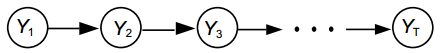
\includegraphics[scale=0.7]{markov-network}
\end{figure}


\begin{definition}
	Las definiciones de los elementos de una red bayesiana dinámica son:
	
	\begin{enumerate}
		\item Sea $\mathcal{Z}=\{Z_{1},...,Z_{N}\}$ un conjunto de variables
		aleatorias que toman valores en función del tiempo, es decir cada
		variable $Z_{k}$ toma valores en $t\ $denotado $Z_{k}(t).$ Denotemos al
		conjunto de variables en el instante $t$ como $\mathcal{Z}%
		[t]=\{Z_{1}(t),...,Z_{N}(t)\}.$
		
		\item Sea $B_{1}$ una red bayesiana sobre las variables $\mathcal{Z}[1]$, la
		cual define la función de distribución de probabilidades conjunta en
		el tiempo inicial denotada por $\mathbb{P}(\mathcal{Z}[1]).$
		
		\item Sea $B_{\Delta }$ una red bayesiana de dos \emph{slices}, la cual
		define la función de distribución de probabilidades condicional de
		la transición del sistema denotada por $\mathbb{P}(\mathcal{Z}[t]\ |\ 
		\mathcal{Z}[t-1]).$
		
		\item Se dice que el par $BD=(B_{1},B_{\Delta })$ es una red bayesiana din%
		ámica.
	\end{enumerate}
\end{definition}

\begin{remark}
	Dependiendo del objetivo del modelo, el conjunto de variables se puede
	particionar en $\mathcal{Z}=(\mathcal{U},\mathcal{X},\mathcal{Y})$,
	conjuntos denotados como \emph{input} (variables de \emph{control}), \emph{%
		hidden} (variables \emph{ocultas}) y \emph{output} (variables \emph{%
		observadas)}.
\end{remark}

\begin{figure}
	\centering
	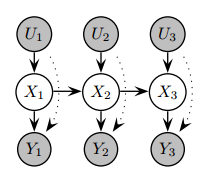
\includegraphics[scale=0.7]{input-hidden-output}
\end{figure}

\begin{proposition}
	Dada una red bayesiana dinámica $BD,$ entonces su función de
	distribución de probabilidades conjunta está dada por: 
	\begin{equation*}
	\mathbb{P}(\mathcal{Z}[1],...,\mathcal{Z}[T])=\prod\limits_{t=1}^{T}\prod%
	\limits_{i=1}^{N}\mathbb{P}_{\Pi }(Z_{i}(t))
	\end{equation*}
\end{proposition}

Como podemos observar, una red bayesiana dinámica esencialmente una red bayesiana con un estado inicial y la transición de estados consecutivos, permitiendo \emph{desenrollar} la red a lo largo del tiempo, resultando un caso particular de red bayesiana. Esto implica que los métodos de entrenamiento y de inferencia para redes bayesianas aplican para redes bayesianas dinámicas, salvo tecnicismos que no afectan mayormente los resultados. En las siguientes secciones vamos a revisar los distintos métodos de entrenamiento y de inferencia para los distintos casos de redes bayesianas.



\subsection{Espacios de Modelos}

La tarea de \emph{learning} es el de inducir un modelo a partir de los datos y del conocimiento \emph{a priori} que se tiene sobre la estructura de los modelos: nodos, arcos, distribuciones y sus parámetros. Este conocimiento inicial es representado como una distribución de probabilidades \emph{a priori }sobre el espacio de modelos, el cual es actualizado usando los datos para obtener una distribución de probabilidades \emph{a posterior} sobre el espacio de modelos. Formalmente, se tienen las siguientes definiciones:

\begin{itemize}
	\item $\mathcal{M}:$ Espacio de estructuras de modelos.
	
	\item $\theta :$ Parámetros de un modelo.
	
	\item $\mathcal{D}:$ Conjunto de datos.
	
	\item $\mathbb{P}(\mathcal{M}):$ Distribución \emph{a prior} de las
	estructuras.
	
	\item $\mathbb{P}(\theta \ |\mathcal{M}):$ Distribución \emph{a prior }%
	de los parámetros dada una estructura.
	
	\item $\mathbb{P}(\mathcal{D}\ |\ \theta ,\mathcal{M}):$ Verosimilitud de
	los datos dada una estructura y sus parámetros.
	
	\item $\mathbb{P}(\mathcal{M}\ |\ \mathcal{D}):$ Distribución \emph{a
		posterior} de los modelos dado los datos:%
	\begin{equation*}
	\mathbb{P}(\mathcal{M}\ |\ \mathcal{D})=\frac{\mathbb{P}(\mathcal{D}\ |\ 
		\mathcal{M})\mathbb{P}(\mathcal{M})}{\mathbb{P}(\ \mathcal{D})}=\frac{\ 
		\mathbb{P}(\mathcal{M})}{\mathbb{P}(\mathcal{D})}\int \mathbb{P}(\mathcal{D}%
	\ |\ \theta ,\mathcal{M})\mathbb{P}(\theta \ |\ \mathcal{M})d\theta
	\end{equation*}
	
	\item $\mathbb{P}(\theta \ |\ \mathcal{M},\mathcal{D}):$ Distribución 
	\emph{a posterior} de los parámetros dada una estructua y los datos:%
	\begin{equation*}
	\mathbb{P}(\theta \ |\ \mathcal{M},\mathcal{D})=\frac{\mathbb{P}(\mathcal{D}%
		\ |\ \theta ,\mathcal{M})\mathbb{P}(\theta \ |\mathcal{M})}{\mathbb{P}(%
		\mathcal{D}\ |\mathcal{M})}
	\end{equation*}
\end{itemize}

Usando las definiciones anteriores, existen diferentes enfoques para el entrenamiento, de los cuales podemos clasificarlos según las siguientes propiedades:

\begin{enumerate}
	\item \emph{Entrenamiento de Parámetros o de Estructuras}: Entrenamiento	de estructuras (usualmente conocido como selección o inducción de modelos) se refiere a aprender la topología del grafo, independiente de la parametrización utilizada, mientras que el entrenamiento de pará metros es de una estructura dada. Puede considerarse que la familia de distribuciones del modelos son parte de la estructura o parte de los pará metros.
	
	\item \emph{Observación Completa o Parcial}: Observación completa se da en el caso que se tienen acceso a todos los datos de todas las variables	del modelo, mientras que observación parcial se da cuando hay datos faltantes o cuando el modelo tiene nodos ocultos.
	
	\item \emph{Estimación Frecuentista o Bayesiana}: La estimación 	frecuentista trata de aprender un único mejor modelo, mientras que la estimación bayesiana trata de aprender una distribución sobre los
	modelos.
	
	\item \emph{Modelos Estáticos o Dinámicos}: Los modelos estáticos son aquellos que no varían en el tiempo, tales como las redes bayesianas, mientras que los modelos dinámicos son aquellos que manejan la variable tiempo de forma especial. Todos los métodos estáticos
	pueden ser aplicados a ambos cosas, pero existen métodos particulares para los casos dinámicos.
	
	\item \emph{Algoritmos Online u Offline}: Los algoritmos \emph{offline} estiman los modelos usando un grupo de datos fijo, mientras que los algoritmos \emph{online} actualizan secuencialmente los modelos a medida que se obtienen nuevos datos.
\end{enumerate}





\subsection{ML: Estimador de máxima verosimilitud}

Dado el conjunto de variables $\mathcal{Z}=\{Z_{1},...,Z_{N}\}$, el caso más simple es asumir que la estructura $\mathcal{M}$ está fija y es dada a priori, y que tenemos observación completa sobre el conjunto de datos $\mathcal{D}=\{D_{1},...,D_{T}\},$ donde $D_{t}=(Z_{1}(t),...,Z_{N}(t)) $ es el vector de valores en el instante $t$. Se define la función \emph{likelihood} (verosimilitud) de los datos $\mathcal{D}$\ sobre los parámetros $\theta =(\theta _{1},...,\theta_{N}) $ como:

\begin{equation*}
\mathbb{P}(\mathcal{D}\ |\ \theta ,\mathcal{M})=\prod\limits_{t=1}^{T}%
\mathbb{P}(D_{t}\ |\ \theta ,\mathcal{M})
\end{equation*}

Por notación, vamos a considerar la dependencia de la estructura está implícita. La estimación de máxima verosimilitud \emph{ML} se obtiene al maximizar la función \emph{likelihood} o equivalentemente la función \emph{log-likelihood:}

\begin{equation*}
L(\theta )=\log \mathbb{P}(\mathcal{D}\ |\ \theta
)=\sum\limits_{t=1}^{T}\sum\limits_{i=1}^{N}\log \mathbb{P}_{\Pi }(Z_{i}(t)\
|\ \theta _{i})
\end{equation*}

Como podemos observar, el máximo se puede calcular de forma local, ya que a cada nodo $Z_{i}$ le corresponde el parámetro $\theta _{i}$, por lo que obtenemos $N$ ecuaciones de la forma

\begin{equation*}
\frac{\partial L}{\partial \theta _{i}}=\sum\limits_{t=1}^{T}\frac{1}{%
	\mathbb{P}_{\Pi }(Z_{i}(t)\ |\ \theta _{i})}\frac{\partial \mathbb{P}_{\Pi
	}(Z_{i}(t)\ |\ \theta _{i})}{\partial \theta _{i}}=0
\end{equation*}



\subsection{MAP: Estimador máximo a posteriori}

Si al caso anterior agregamos una ditribución \emph{a priori} sobre los parámetros $\theta $, entonces la estimación de máxima a posteriori \emph{MAP} se obtiene al maximizar la función análoga al caso \emph{ML}:

\begin{equation*}
L(\theta )=\log \mathbb{P}(\mathcal{D}\ |\ \theta )\mathbb{P}(\theta
)=\sum\limits_{t=1}^{T}\sum\limits_{i=1}^{N}\log \mathbb{P}_{\Pi }(Z_{i}(t)\
|\ \theta _{i})+\sum\limits_{i=1}^{N}\log \mathbb{P}(\theta _{i})
\end{equation*}


Si denotamos $\mathcal{D}$ al conjunto de datos disponibles y $\theta $ al conjunto de parámetros que deseamos estimar, entonces la distribución \emph{a posteriori} de los parámetros está dada por:

\begin{equation*}
\mathbb{P}(\theta \ |\ \mathcal{D})=\frac{\mathbb{P}(\mathcal{D}\ |\ \theta )%
	\mathbb{P}(\theta )}{\mathbb{P}(\mathcal{D})}\varpropto \mathbb{P}(\mathcal{D%
}\ |\ \theta )\mathbb{P}(\theta )
\end{equation*}

$\mathbb{P}(\mathcal{D}\ |\ \theta )$ denota la \emph{verosimilitud} de los datos $\mathcal{D}$ dados los parámetros $\theta $, y $\mathbb{P}(\theta)$ denota la distribución \emph{a priori} de los parámetros $\theta
. $ La etapa de entrenamiento busca maximizar la distribución \emph{a posteriori} $\mathbb{P}(\theta \ |\ \mathcal{D}),$ o en el caso que no se haga ninguna suposición sobre los parámetros $\theta $, busca
maximizar la \emph{verosimilitud}$\mathbb{\ P}(\mathcal{D}\ |\ \theta ).$

En el caso general denotamos $Z=\{Z_{1},...,Z_{n}\}$ al conjunto de variables de la red, entonces el conjunto $\mathcal{D}$ contiene $M$ tuplas que asigna un valor a cada variable, por lo que podemos expresar
\begin{equation*}
\mathbb{P}(\mathcal{D}\ |\ \theta )=\prod\limits_{i=1}^{M}\mathbb{P}%
(D^{(i)}\ |\ \theta )
\end{equation*}

Para obtener el $\arg \max_{\theta }$ $\mathbb{P}(\theta \ |\ \mathcal{D})$, podemos maximizar directamente la función \emph{likelihood} o equivalentemente \emph{log-likelihood}

\begin{equation*}
L(\theta )=\log \mathbb{P}(\theta \ |\ \mathcal{D})=\sum_{i=1}^{M}\log 
\mathbb{P}(D^{(i)}\ |\ \theta )+\log \mathbb{P}(\theta )
\end{equation*}

Si los datos están completos, es decir $D^{(i)}=\{z_{1}^{(i)},...,z_{n}^{(i)}\}$ para todo $i=1...n,$ entonces la función se puede simplificar como

\begin{equation*}
L(\theta )=\sum_{i=1}^{M}\sum_{j=1}^{n}\log \mathbb{P}(z_{j}^{(i)}|\ \Pi
(z_{j}^{(i)}),\theta )+\log \mathbb{P}(\theta )
\end{equation*}

donde $\Pi (z_{j}^{(i)})$ denota el conjunto de variables padres de $z_{j}$ con su respectiva asignación de valores en $D^{(i)}.$ De esta forma, podemos maximizar $L(\theta )$ utilizando esta fórmula explícita. El caso de redes bayesianas dinámicas es bastante similar, pero en vez de tener $M$ tuplas de datos se tienen $T$ periodos consecutivos de datos, siendo una fórmula análoga.

En el caso que los datos no están completos, la situación cambia abruptamente, ya que no es posible dejar la fórmula de una forma explícita, por lo que se propone seguir un enfoque distinto. Por simplicidad vamos a omitir el término $\mathbb{P}(\theta )$ en el resto del capítulo, ya que incluirlo es bastante directo.



\subsection{EM: Algoritmo de Expectation-Maximization}

Denotemos $X$ al conjunto de variables ocultas y denotemos $Y$ al conjunto de variables observables, es decir $D^{(i)}=\{y_{1}^{(i)},...,y_{n_{y}}^{(i)}\}.$ Entonces la función \emph{log-likelihood} es la siguiente

\begin{equation*}
L(\theta )=\log \mathbb{P}(\mathcal{D}\ |\ \theta
)=\sum\limits_{i=1}^{M}\log \int_{X}\mathbb{P}(X,D^{(i)}\ |\ \theta )dX
\end{equation*}

A diferencia del caso de observación completa, esta función no es posible descomponerla en sumas locales por nodos. Una técnica posible es utilizar la \emph{desigualdad de Jensen} para obtener una cota inferior de la función \emph{log-likelihood}.

\begin{theorem}
	Dado un espacio de probabilidades, toda función concava $f$ y toda función $g$ $\mathbb{P}$-medible se cumple que 
	\begin{equation*}
	f\left( \int\limits_{\Omega }g\ d\mathbb{P}\right) \geq \int\limits_{\Omega
	}f\circ g\ d\mathbb{P}
	\end{equation*}
\end{theorem}

Intuitivamente, el resultado anterior dice que $f$ del promedio de $g$ es mayor que el promedio de $f$ de $g$. Como la función $\log $ es cóncava, y usando cualquier distribución $Q$ sobre las variables ocultas $X$, podemos aplicar la \emph{desigualdad de Jensen} de la siguiente forma:

\begin{eqnarray*}
	L(\theta ) &=&\log \int_{X}\mathbb{P}(X,Y\ |\ \theta )dX \\
	&=&\log \int_{X}Q(X)\frac{\mathbb{P}(X,Y\ |\ \theta )}{Q(X)}dX \\
	&\geq &\int_{X}Q(X)\log \frac{\mathbb{P}(X,Y\ |\ \theta )}{Q(X)}dX \\
	&=&\int_{X}Q(X)\log \mathbb{P}(X,Y\ |\ \theta )dX-\int_{X}Q(X)\log Q(X)dX \\
	&=&\mathcal{F}(Q,\theta )
\end{eqnarray*}

Podemos ver que $\mathcal{F}(Q,\theta )$ es una cota inferior de $L(\theta )$, por lo que es razonable pensar que una opción es maximizar $\mathcal{F}(Q,\theta )$. El algoritmo \emph{EM} (\emph{Expectation Maximization)} busca maximizar $\mathcal{F}$, alternando de forma iterativa entre dos etapas, partiendo desde un parámetro inicial $\theta _{0}:$

\begin{eqnarray*}
	\emph{E\ step}\emph{:\ } &&Q_{k+1}\leftarrow \arg \max\limits_{Q}\mathcal{F}
	(Q,\theta _{k}) \\
	\emph{M\ step}\emph{:\ } &&\theta _{k+1}\leftarrow \arg \max\limits_{\theta }
	\mathcal{F}(Q_{k},\theta )
\end{eqnarray*}

Un resultado conocido en la literatura nos simplifica el paso \emph{E}, ya que
\begin{equation*}
Q_{k+1}(X)=\mathbb{P}(X\ |\ Y,\theta _{k})
\end{equation*}

Eso implica que cada iteración se puede escribir como

\begin{equation*}
\emph{EM\ step}\emph{:}\emph{\ }\theta _{k+1}\leftarrow \arg
\max\limits_{\theta }\int_{X}\mathbb{P}(X\ |\ Y,\theta _{k})\log \mathbb{P}%
(X,Y\ |\ \theta )dX
\end{equation*}

El siguiente resultado sobre la convergencia de los pasos de \emph{EM} muestran la validez del algoritmo \emph{EM}.

\begin{theorem}
	\emph{(Dempster et al., 1977)} El algoritmo \emph{EM} incrementa $L(\theta )$
	en cada iteración:
	\begin{equation*}
	L(\theta _{k+1})\geq L(\theta _{k})
	\end{equation*}
	
	donde la igualdad se alcanza
	\begin{equation*}
	L(\theta _{k+1})=L(\theta _{k})\Longleftrightarrow \mathbb{P}(X\ |\ Y,\theta
	_{k+1})=\mathbb{P}(X\ |\ Y,\theta _{k})
	\end{equation*}
\end{theorem}

\begin{definition}
	De ahora en adelante vamos a denotar
	\begin{equation*}
	Q(\theta ;\theta _{k})=\int_{X}\mathbb{P}(X\ |\ Y,\theta _{k})\log \mathbb{P}
	(X,Y\ |\ \theta )dX
	\end{equation*}
\end{definition}

Es posible relajar la condición de buscar el máximo, ya que basta con encontrar $\theta _{k+1}$ tal que $Q(\theta _{k+1};\theta _{k})\geq Q(\theta _{k};\theta _{k})$ para que el resultado anterior siga siendo válido$.$ Esta versión relajada del algoritmo se conoce como \emph{Generalized Expectation Maximization}.

\begin{figure}
	\centering
	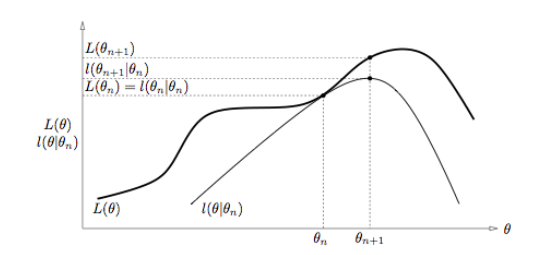
\includegraphics[scale=0.7]{EM}
\end{figure}

\subsection{EM Estocástico}

El algoritmo \emph{EM} nos da un método para estimar los parámetros $\theta $ de nuestro modelo de una forma clara y con fundamentos sólidos. El gran problema de este enfoque es calcular la función $Q(\theta;\theta _{k})$ en el caso general:

\begin{equation*}
Q(\theta ;\theta _{k})=\int_{X}\mathbb{P}(X\ |\ Y,\theta _{k})\log \mathbb{P}
(X,Y\ |\ \theta )dX=\mathbb{E}_{\mathbb{P}(X\ |\ Y,\theta _{k})}\mathbb{(}
\log \mathbb{P}(X,Y\ |\ \theta )\mathbb{)}
\end{equation*}

Salvo casos particulares, no es posible calcular de forma exacta esta esperanza, ya que a pesar que a la distribución $\mathbb{P}(X,Y\ |\theta )$ podemos aplicar la regla de la cadena para obtener una expresión más simple, no podemos realizar ninguna simplificación analítica a $\mathbb{P}(X\ |\ Y,\theta _{k})$.

Una opción razonable es calcular la esperanza utilizando algún método de \emph{Monte Carlo}:
\begin{eqnarray*}
	\mathbb{E}_{\mathbb{P}(X\ |\ Y,\theta _{k})}\mathbb{(}\log \mathbb{P}(X,Y\
	|\ \theta )\mathbb{)} &\mathbb{\approx }&\frac{1}{N_{k}}\sum_{i=1}^{N_{k}}%
	\log \mathbb{P}(X_{k}^{(i)},Y\ |\ \theta ) \\
	X_{k}^{(i)} &\sim &\mathbb{P}(X\ |\ Y,\theta _{k})\text{ }i=1...N_{k}
\end{eqnarray*}

Como pudimos revisar en el capítulo anterior sobre \emph{inferencia}, obtener el conjunto de \emph{samples} $\{X_{k}^{(i)}\}_{i=1}^{N_{k}}$ no es para nada trivial y puede requerir realizar alguna aproximación de la distribución real. El algoritmo general agrega un paso adicional a los ya conocidos \emph{E} y \emph{M}, y es el paso \emph{S} que se refiere al paso \emph{Simulation} para obtener los \emph{samples}. Cuando en el paso $\emph{S}$ se obtiene una única muestra se conoce como \emph{Stochastic EM (StEM)}, y si se realiza algún método basado en \emph{Monte Carlo} se conoce como \emph{Monte Carlo EM}. 


La estimación se basa en que las iteraciones del algoritmo \emph{StEM}
es una cadena de Markov que converge a una distribución estacionaria de
los parámetros $\theta $, por lo que luego del periodo de \emph{burn-in}%
, los parámetros $\theta $ pueden ser estimados al promediar la
secuencia de parámetros de cada iteración de \emph{StEM}.

Existen otras modificaciones del algoritmo base, por ejemplo \emph{%
	Stochastic Approximation EM (SAEM)} realiza una aproximación estocá%
stica iterativa de $Q(\theta ;\theta _{k})$ de la siguiente forma%
\begin{equation*}
Q(\theta ;\theta _{k})\approx \hat{Q}_{k}(\theta )=(1-\gamma _{k})\hat{Q}%
_{k-1}(\theta )+\gamma _{k}(\frac{1}{N_{k}}\sum_{i=1}^{N_{k}}\log \mathbb{P}%
(X_{k}^{(i)},Y\ |\ \theta ))\text{ }
\end{equation*}

donde $\{\gamma _{k}\}_{k\geq 1}$ es una secuencia decreciente tal que $\sum\gamma _{k}=\infty $ y $\sum \gamma _{k}^{2}<\infty$. La idea de esta aproximación es ser más eficiente en cada paso, ya que se muestra que esta variación tiene un buen comportamiento incluso si se considera $N_{k}=1$, ya que todas las simulaciones del pasado contribuyen a la estimación actual, pero van perdiendo peso en cada iteración.


\subsection{Recocido determinista de EM}

Los métodos de la sección anterior tienen el problema que pueden converger a mínimos locales, alejándose considerablemente del óptimo global. Un enfoque es el de iterar el algoritmo base multiples veces, partiendo desde distintos puntos iniciales, para finalmente considerar la mejor estimación de todas las obtenidas. El problema de este enfoque es que es muy costoso computacionalmente, además que está completamente acondicionada al conjunto de puntos iniciales seleccionados.

Una alternativa mucho más eficiente es usar la técnica conocida como \emph{deterministic annealing (DA)}, la cual se basa en aplicar un cierto nivel de \emph{entropía} (ruido) en el sistema, el cual se reduce gradualmente. En la sección anterior obtuvimos una cota inferior de la forma:

\begin{equation*}
\mathcal{F}(Q,\theta )=\int_{X}Q(X)\log \mathbb{P}(X,Y\ |\ \theta
)dX-\int_{X}Q(X)\log Q(X)dX
\end{equation*}

Desde un punto de vista análogo a la mecánica estadística, el primer término corresponde a la \emph{energía libre} del sistema, mientras que el segundo término corresponde a la \emph{entropía}. La idea detrás de \emph{DA} es multiplicar la \emph{entropía} por un término $T$ correspondiente a la \emph{temperatura} del sistema; inicialmente la \emph{temperatura} es alta, la cual \emph{suaviza} la superficie de la \emph{energía libre}, por lo cual es fácil encontrar el máximo; luego la temperatura es reducida gradualmente a $T=1,$ convergiendo al problema original. Si la \emph{temperatura} es reducida lo suficientemente lenta, es posible rastrear el óptimo global.

El algoritmo \emph{DAEM} (\emph{Deterministic Annealing Expectation Maximization)} es una variación \emph{DA} del algoritmo \emph{EM}, alternando de forma iterativa entre dos etapas, partiendo desde un parámetro inicial $\theta _{0}$ y un $\beta \in \lbrack 0,1],$ con una función $g$ que incremente $\beta $ suavemente hasta $1$, se obtiene:

\begin{eqnarray*}
	\emph{E\ step}\emph{:\ } &&Q_{k+1}^{\beta }\leftarrow \frac{\mathbb{P}(X,Y\
		|\ \theta _{k})^{\beta }}{\int_{X}\mathbb{P}(X,Y\ |\ \theta _{k})^{\beta }dX}
	\\
	\emph{M\ step}\emph{:\ } &&\theta _{k+1}\leftarrow \arg \max\limits_{\theta
	}\int_{X}Q_{k+1}^{\beta }\log \mathbb{P}(X,Y\ |\ \theta )dX \\
	\text{{}}\beta \ \text{\emph{step}} &\emph{:}&\text{\ }\beta \leftarrow
	g(\beta )
\end{eqnarray*}

Para poder calcular la fórmula usando alguno de los métodos de \emph{Monte Carlo}, podemos expresar $Q_{\beta}(\theta ;\theta _{k})$ como:

\begin{eqnarray*}
	Q_{\beta }(\theta ;\theta _{k}) &=&\frac{1}{\int_{X}\mathbb{P}(X,Y\ |\
		\theta _{k})^{\beta }dX}\int_{X}\frac{\mathbb{P}(X\ |\ Y,\theta _{k})}{
		\mathbb{P}(X\ |\ Y,\theta _{k})}\mathbb{P}(X,Y\ |\ \theta _{k})^{\beta }\log 
	\mathbb{P}(X,Y\ |\ \theta )dX \\
	&=&\frac{\mathbb{P}(Y\ |\ \theta _{k})}{\int_{X}\mathbb{P}(X,Y\ |\ \theta
		_{k})^{\beta }dX}\int_{X}\mathbb{P}(X\ |\ Y,\theta _{k})\frac{\mathbb{P}
		(X,Y\ |\ \theta _{k})^{\beta }}{\mathbb{P}(X,Y\ |\ \theta _{k})}\log \mathbb{
		P}(X,Y\ |\ \theta )dX \\
	&=&C_{k,\beta }\int_{X}\mathbb{P}(X\ |\ Y,\theta _{k})\frac{\log \mathbb{P}
		(X,Y\ |\ \theta )}{\mathbb{P}(X,Y\ |\ \theta _{k})^{1-\beta }}dX \\
	&\approx &C_{k,\beta }\sum_{i=1}^{N_{k}}\frac{w_{k}^{(i)}}{\mathbb{P}
		(X_{k}^{(i)},Y\ |\ \theta _{k})^{1-\beta }}\log \mathbb{P}(X_{k}^{(i)},Y\ |\
	\theta ) \\
	C_{k,\beta } &=&\left[ \sum_{i=1}^{N_{k}}\frac{w_{k}^{(i)}}{\mathbb{P}
		(X_{k}^{(i)},Y\ |\ \theta _{k})^{1-\beta }}\right] ^{-1}
\end{eqnarray*}

Más detalles de este algoritmo, sus tecnicismos y su fundamento teórico se puede encontrar en \cite{DBN-DAEM}.
